\section{Structure of communication protocols}
\label{sec:structure_protocols}

Before getting into more details about the search and implementation of the surveyed protocols, the structure and functionality of communication protocols is described. This is for the sake of clarity to the readers and the author himself. Without a thorough understanding of a protocol structure and what to expect from it, the requirements could be misinterpreted, resulting in erroneously grounded research. This section is especially beneficial for new or less experienced readers on this subject.

\subsection{The OSI model}
Communication functions of a computer system can be developed keeping the standardized Open Systems Interconnection (OSI) \cite{OSImodel} model in mind. This model is designed to describe how data communication between two peers should take place. According to the OSI model communication systems consist of seven different layers which can be interpreted as groups with their own functions and responsibilities. In short, the model defines a stack of standards describing the way devices communicate and inform each other, when to send data, when to stop transmitting data, and so on. It also ensures devices use the correct data rate, guarantees the arrival of data at the receiver side, and in which way the physical connection is implemented.
A general overview of the seven layers can be seen in Figure~\ref{Fig:Osimodel}~\cite{OSImodel}. The depicted structure goes bottom up with the lowest layer below.

\begin{figure}[H]
	\centering
	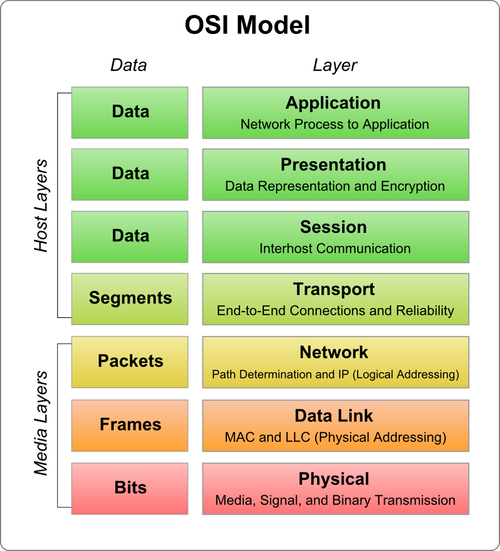
\includegraphics[width=0.45\textwidth]{osimodel.png}	
	\caption{An overview of the OSI model.}
	\label{Fig:Osimodel}
\end{figure}

The first layer is the \textit{physical layer} which is responsible for the communication signals passing through the connection between two points. Often the term \textit{PHY} is used to refer to this layer. This concerns the physical connectors, cables, pin-outs and also the actual voltage (or the light) on the line, depending on the type of encoding the protocol makes use of. As shown in the figure above, the data from this layer can be seen as multiple "raw" bits. Further specifications the physical layer normally includes are the data rates, maximum transmission distances and low-level error correction.
For example in the Ethernet standard this layer contains multiple sub-layers which are the Physical Coding Sub-layer (PCS) delivering encoded data, Physical Medium Attachment Sub-layer (PMA) responsible for the attachment interface, Physical Medium Dependent Sub-layer (PMD) which defines the electrical transmit/receive characteristics and the Forward Error Correction Sub-layer (FEC)~\cite{EthernetPHY}.\\

The second layer is called the \textit{data link layer} and ensures error-free data transmission between two physical layers. This is done by arranging the stream of data in such way the receiver can easily understand. This is done by packing the data into so called frames, an explanation of which will follow in section \ref{subsec:framing}. These frames will then be moved to the physical layer. This layer is also responsible for computing and adding data error correction, and including framing bits.  
The layer can also be divided in two sub-layers, the Logical Link Control (LLC) and the Media Access Control (MAC). The LLC is responsible for error checking, frame synchronization and flow control while the MAC is responsible for controlling how multi-peer network access is granted to the medium, and the permission to transmit data.\\

The third layer is the \textit{network layer} which is primarily responsible for determining which physical path the data should take. It contains the function to route the data to it's recipient according to circumstances. This is where addresses will be added to the packets which is comparable with the well-known IP addressing from the Internet Protocol Suite~\cite{OSI_IP/TCP/UDP}. Other functions handled by the data layer are packet switching and sequence control.\\

The fourth layer is called the \textit{transport layer} and here the focus lies more on the delivery of messages between networked hosts. This is where the messages are fragmented and reassembled. This also contains higher-level error detection and recovery, flow control and guaranteed data delivery. Common protocols that function on this layer are TCP and UDP~\cite{OSI_IP/TCP/UDP}.\\

Since this document intends to target chip-to-chip communication, not all layers are important. In this case the Physical and Data Link layers are of most interest. Networking is also interesting in case data has to be transmitted over multiple channels. The transport layer can be of interest in case of multi-peer networked topologies, and that is the reason why it was still described. The other layers are of less interest. 

\subsection[Data structure and framing]{Data structure and framing \hfill OSI Layer 2}
\label{subsec:framing}
Transferring data is not just transmitting a bulk of data bytes to the other side. A certain amount of bytes will be accepted by the protocol which will package this data and prepare this for transmission. Depending on the protocol users can indicate when the data stream starts and when this ends. A whole lot of other indicators could be available to the user like choosing which bytes in the specific package are valid or the channel number to transmit on in the case of multiple data lines. The protocol will register this and pack them into so called frames.\cite{Framing}

Not only do these frames contain for example the start and end of a package but they could also be used to transmit error correction and other crucial information. These frames are often categorized as control words. However the data itself is packed in a data word. These words always contain the same amount of bits. \cite{InterlakenProtocol} \\

Of course the data can be transferred using a serial or parallel connection. This completely depends on what the designer of the protocol has implemented and at which speed the data is required to be transferred. Transmitting data in parallel requires more effort in comparison to a serial connection but delivers more data to the other side in the same time as expected. The data itself can be serially processed inside the electronics but it is also possible to process this in parallel using a specific package width. 

\subsection[Error detection and correction]{Error detection and correction \hfill OSI Layer 2/1}
It is never certain whether the data received exactly matches the data that has been transmitted. During the data transmission all kinds of interference can be picked up by the communication line and can cause data bits to flip or be read as the wrong binary value. Without any indication whether these events overcame the data this bit flip will go unnoticed and corrupt data will be processed as if it were identical to the data sent by the transmitter.

To overcome these unnoticed forms of data corruption multiple ways of so called error correction have been researched and are nowadays nearly always implemented. The only downside of error correction is that additional information has to be transmitted between data packets but this sacrifice is in most cases worth the guarantee correct data will be processed by the receiver.\\

The easiest way of error detection is to add a checksum making use of a parity check. In this case the total number of high bits will represent a value according to their position in a specific byte. These values will be summed and the total will be divided by the amount of bytes again. This method offers easy detection of a single bit flip but if two bits are flipped at the same position in two different words, which represent the same value, the checksum won't change. For small amounts of data which are not that important it should suffice but when the received data is has a more important function, other methods of error detection are preferred.\\

Another form is the Cyclic Redundancy Check (CRC) which has to be implemented before the encoding of data. In this case a so called polynomial is implemented which will be used as a divisor on the data. This pack of data will be divided by the polynomial starting at the most significant bit. After every division the result will be divided again but this time with the divisor shifted one position to the left. This can be interpreted as constantly using an XOR on the data bits. At the end of constant divisions, the complete data pack itself will be padded with zeros while the remainder should be the length of the divisor minus one bit. While dividing it is important to know that when the leftmost bit of the result data equals zero, the data will be divided by zeros instead of the divisor.

To validate the data this complete division will be repeated again but now using the generated remainder. This should result in is exactly zero for both the resulted data and remainder. \cite{CRCLB} When the result is not equal to zero the received data is not identical to the data that was originally transmitted. An example of this check with a correctly arrived and corrupted package is depicted in Figure \ref{fig:CRC_Check}.\cite{CRC1} The most common CRC variants currently in use are CRC-8, CRC-16 and CRC-32. \\

\begin{figure}[ht]
	\centering
	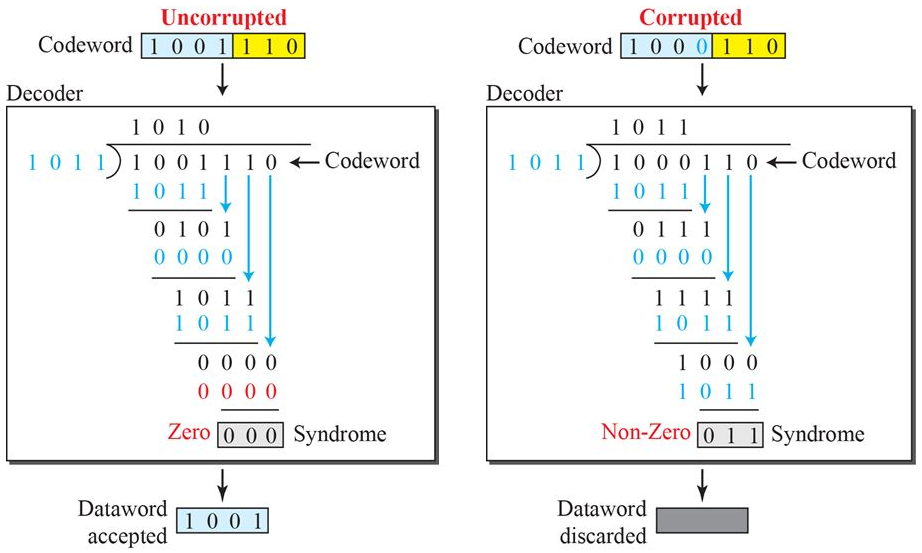
\includegraphics[width=0.65\textwidth]{CRC1.png}	
	\caption{CRC division in case data appears flawless or corrupted.}
	\label{fig:CRC_Check}
\end{figure} 

\label{sec:FEC}
Forward Error Correction (FEC) is also an option which most of the times is used after encoding the data stream. Another term used for this way of error correction is channel coding. This technique is used to detect errors while communicating over unreliable or noisy channels. The big advantage of this technique is that it contains the ability to correct errors and when strategically placed between the encoder and transmission line, data entering the decoder will not contain errors caused during the physical transmission.

The so called Reed-Solomon error correction is an often implemented variant of FEC which contains the ability to detect and correct symbol errors. 
Another high-performance variant of FEC is called turbo code. This specific method of error correction makes use of two encoders, an inner and outer encoder with an additional interleaver. Multiple variants of these turbo codes are in use nowadays which are for example popular in deep space communication, 3G, 4G and different satellite networks. Optical forms of communication also make use of turbo code \cite{turbocode}.

\subsection[Encoding of data]{Encoding of data \hfill OSI Layer 1}
\label{Sub:Structure_Encoding}
Data has primarily always been transmitted using physical electrical conductive connections. While transmitting a lot of the same signs in a row over such a line, this causes the average line voltage to change in value and thus introduces a DC-component. This can cause the capacitance of line filters to be charged and the average voltage between ones and zeros can shift. This will eventually result in corrupt data and can even damage connected components. While the so called baseline wander is problematic, the short on transitions can additionally cause errors in the delineation of word boundaries, a form of constant EMI will be present and clock recovery\footnote{The process of regenerating the clock signal at the receiving side with the absence of a separate clock signal. This can be done by using the timing information of the data stream.} won't be possible since there will be no transitions to focus on. \\

A widely used solution to this problem is the addition of so called line encoding. The purpose of this technique is to encode the data in such way the receiver can still decipher it but long steams of the same binary value will be prevented. Encoders come in a lot of different variants. \\

The most simple and often used variant is 8b/10b encoding. This makes use of certain algorithms that will translate the bits to a specific pattern that will be transmitted. However as the name indicates for every eight bit transmitted two will be added as a header which results in about 20 percent of wasted bandwidth. The reason why they are still used a lot is because of their excellent DC-balance and they are easy to implement.\\

Through time more advanced encoders have developed like the 64B/66B encoder. The caused reason to innovate was primarily because of the overhead included with 8b/10b encoding. Since data rates nowadays grow rapidly, as less bandwidth as possible should be wasted. These moderner encoders also don't use a lookup table but make use of a so called scrambler which uses an algorithm to randomize the bit orders. Multiple variants have again tried to improve on the 64b/66b like the 64b/67b which offers better DC-balance. More details on this subject will be explained in section \ref{sec:encoding_decoding} which will be dedicated to the currently existing ways of encoding and decoding.

\subsection[Serialization and parallelization of data]{Serialization and parallelization of data \hfill OSI Layer 1}
Serial and parallel data streams have been discussed in short earlier. When high speed transmissions are required it is preferred to gain a speed high as possible over a single transmission line. This doesn't mean all data processing operations inside the chips have to happen in serial order. Most of the times data is processed in parallel using FPGA's or dedicated chips suited for data transfer. Serially processing the data steam inside the chips would be too slow and bottleneck the line speed.

The parallel data bus will be translated into one or multiple serial data steams at the transmitter side and the receiver has to revert this transformation. Of course the speed of these lanes will also be altered according to the speed the parallel bus was transferring data on. The component that is responsible for this task is called a "Gearbox". When for example four 2,5 Gbps lanes are translated into a single 10 Gbps line, this would be mentioned as a 4:1 gearbox. The same can be said when this process is reversed with a 1:4 gearbox. Often this conversion block is also called a SerDes (SerializerDeserializer) and this is the last step before transmitting data. In Figure \ref{fig:gearbox} an example of two gearboxes with a transmission line in between is shown. \cite{Gearbox}

\begin{figure}[H]
	\centering
	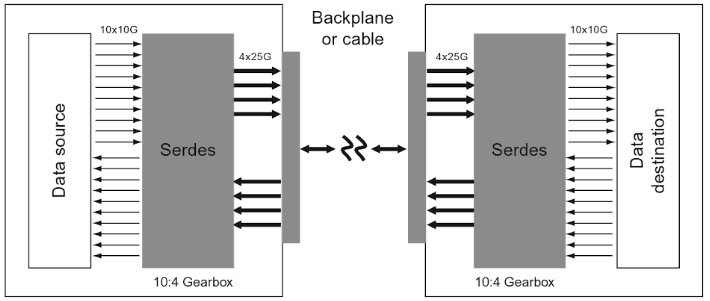
\includegraphics[width=0.8\textwidth]{Gearbox.png}	
	\caption{SerDes gearboxes.}
	\label{fig:gearbox}
\end{figure} 

\newpage
\subsection{Protocol overview}
After this research it should be clearer what to expect of a communication protocol and what fundamental components it consists of. A simple depiction can be made to summarize this section which can be seen in Figure \ref{fig:protocol_overview}. Transmitted and received data will both be stored in separate FIFO's which act as a buffer for adding and removing frames in between the data packets. In case independent clock FIFO's are implemented, the protocol can be assigned different clock speeds than other section on the chip which can be seen as an advantage.

\begin{figure}[H]
	\centering
	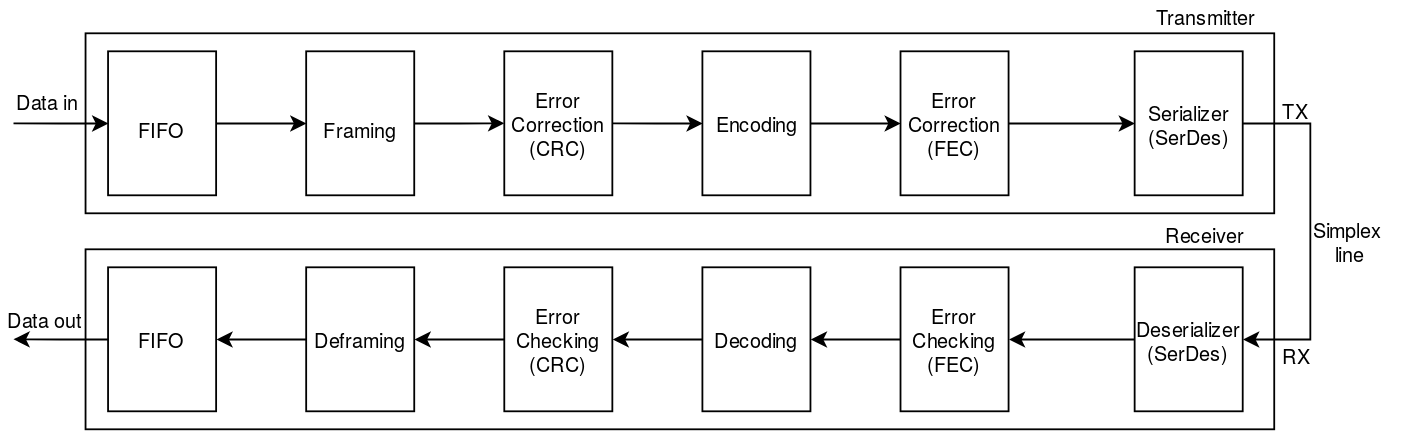
\includegraphics[width=\textwidth]{Protocol_Overview.png}	
	\caption{Protocol overview according to earlier subsections.}
	\label{fig:protocol_overview}
\end{figure} 

The framing, encoding and error checking are also present. In this example a simplex line has been displayed. Data is only transmitted in one direction from TX to RX. Both the transmitting and receiving side should have a TX and RX pin. Additional information and status updates on the receiver can then be transmitted in the other direction. This way data transmission could be for example slowed down or completely stopped in case an error occurs at the receiver side.
\newpage